

\section{Methods}



% \begin{figure*}[t]
%   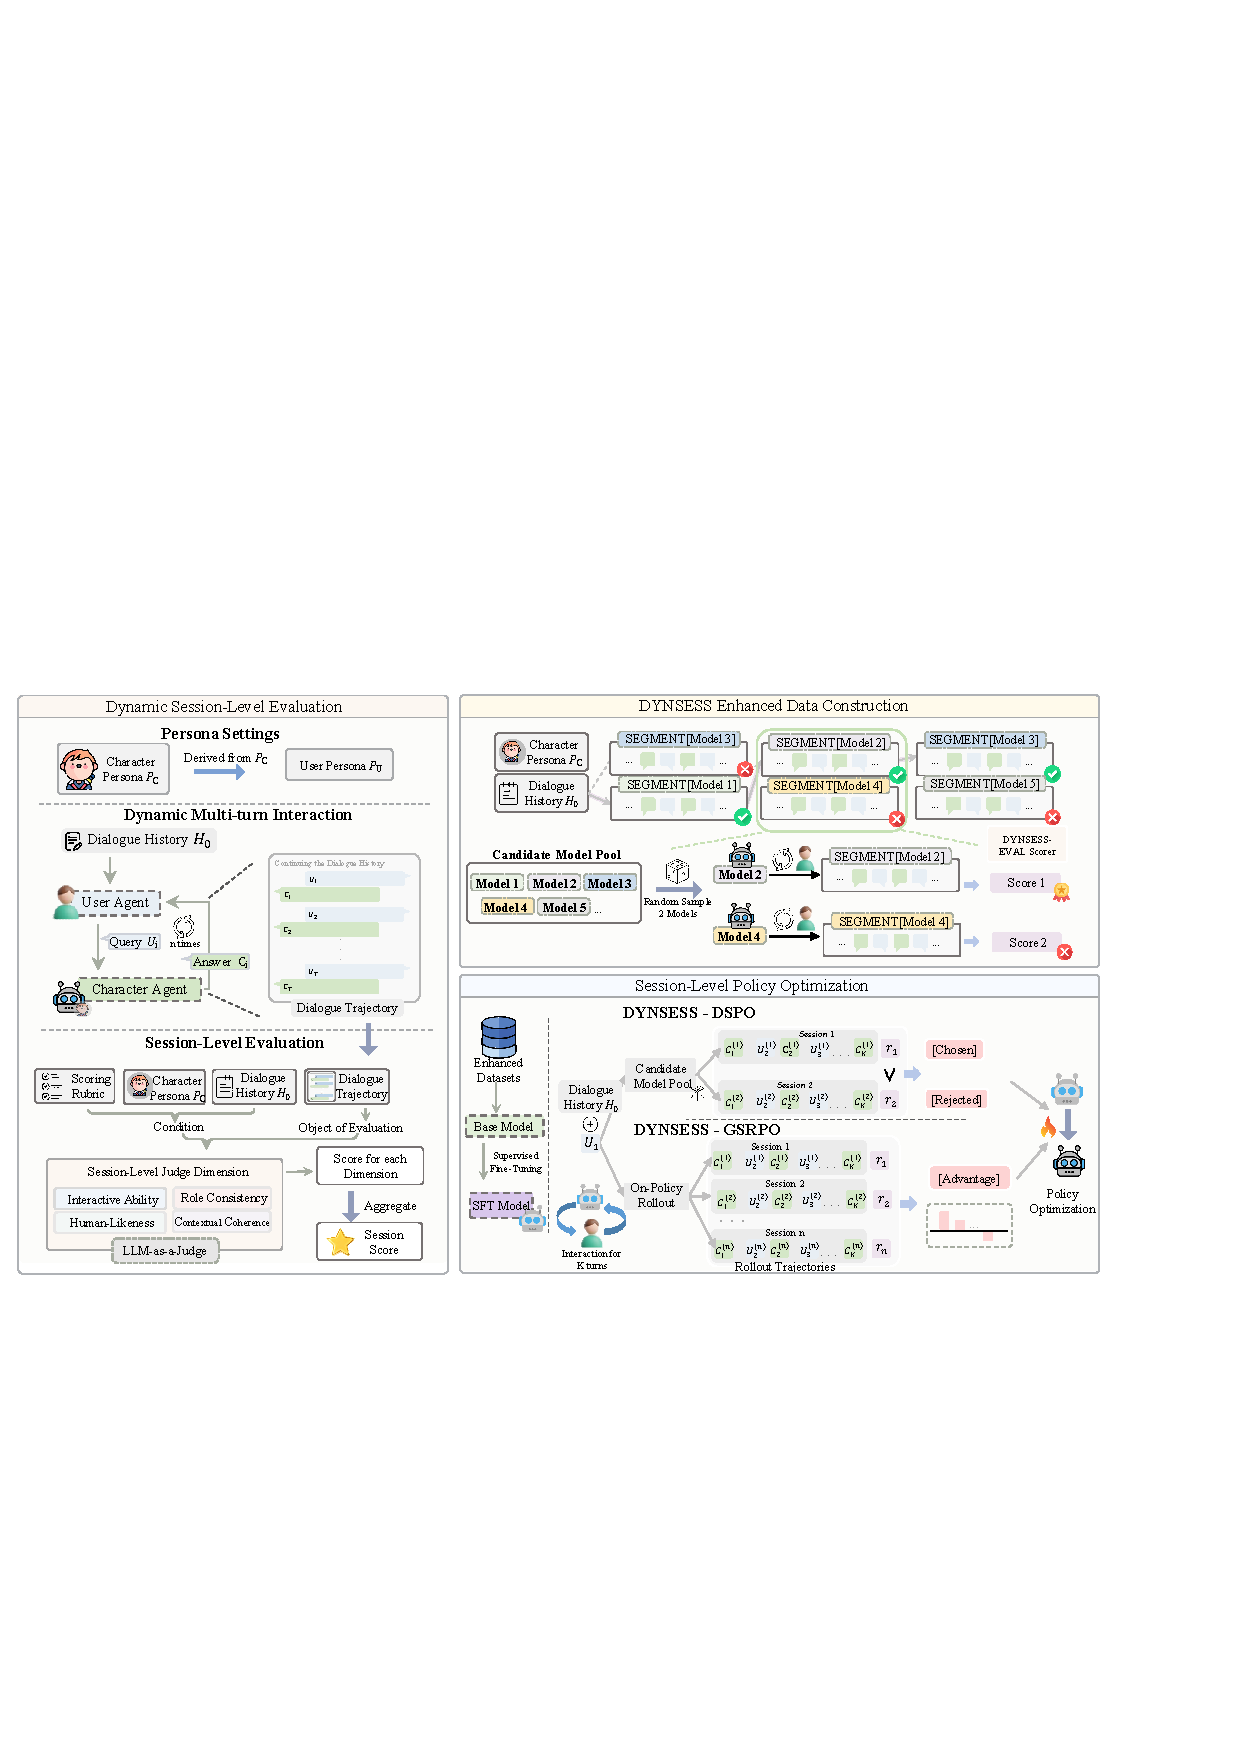
\includegraphics[width=\textwidth, trim = 0 8cm 2cm 11.5cm, clip]{latex/Image/method-0519.pdf}
%   \caption{Overview of DYNSESS-EVAL for session-level evaluation and DynSess-Character for session-level training.}
%   \label{fig:method}
% \end{figure*}


In this section, we present our dynamic session-level framework for role-playing agents (illustrated in Fig.~\ref{fig:method}). As shown on the left side of the figure, DynSess-Eval serves as our evaluation component (detailed in Section \ref{sec:eval}). On the right side, DynSess-Character functions as the optimization module (detailed in Section \ref{sec:train}).



\subsection{Dynamic Session-Level Evaluation}
\label{sec:eval}

We propose Dynamic Session Evaluation (\textbf{DynSess-Eval}) to investigate the long-term conversational capabilities of role-play agents. Our key insight is that turn-level evaluation, which generates a single reply given a fixed history, lacks the longitudinal perspective to track behavioral drift and fails to account for dynamic user engagement. Therefore yields inaccurate assessments of an agent's long-term coherence.

To address this limitation, DynSess-Eval transitions from static evaluation to dynamic interaction by introducing a user simulator. As illustrated in the left panel of Fig.~\ref{fig:method}, an evaluation instance is initialized with a target character persona $P_C$ and an optional initial context $H_0$. 
%As illustrated in the left panel of Fig.\ref{fig:method}, an evaluation instance is initialized with a target character persona $P_C$ and an optional dialogue history $H_0$.
We first synthesize a user persona $P_U$ via a derivation module $\mathcal{M}_{\text{up}}$, parameterized by a prompt template $\mathcal{I}_{\text{up}}$ (see Appendix~\ref{app:prompt_user_persona}):
\begin{equation}
P_U \sim \mathcal{M}_{\text{up}}(\cdot \mid \mathcal{I}_{\text{up}}, P_C).
\end{equation}
Equipped with $P_C$ and $P_U$, we simulate a $T$-turn interactive session between the character agent $\pi_\theta$ and  user simulator $\pi_{\text{user}}$. At each turn $t$, both models generate responses conditioned on their respective personas and the preceding context $H_{t-1}$:
\begin{equation}
\begin{split}
u_t &\sim \pi_{\text{user}}(\cdot \mid P_U, H_{t-1}), \\
a_t &\sim \pi_{\theta}(\cdot \mid P_C, H_{t-1} \oplus u_t),
\end{split}
\end{equation}
where $u_t$ and $a_t$ denote the user utterance and agent response at turn $t$, respectively. The context is incrementally updated by appending the new utterances: $H_t = H_{t-1} \oplus (u_t, a_t)$. The resulting $T$-turn session is denoted as $\tau = H_T$.

\paragraph{Rubric-Anchored Session Scoring.}
Evaluating subjective tasks with standard LLM-as-a-judge prompts often yields inflated and unstable scores, as LLMs struggle to consistently balance multiple criteria across long, multi-turn interactions. Inspired by \cite{wei2025rocketeval}, we propose a \textbf{rubric-anchored judge} J that decouples evidence extraction from score aggregation, providing reliable and interpretable session-level signals.

Following common practices in role-playing evaluation~\cite{zhou2025characterbench}, we assess agents across four dimensions: \textit{Interactive Ability} ($D_{\text{IA}}$), \textit{Human-likeness} ($D_{\text{HL}}$), \textit{Role Consistency} ($D_{\text{RC}}$), and \textit{Contextual Coherence} ($D_{\text{CC}}$). To capture long-term dynamics,  we design dedicated \textbf{session-level criteria} $\mathcal{C}_d$ for each dimension, explicitly targeting long-horizon behaviors such as \textit{gradual persona drift}, \textit{repetitive loops}, and \textit{memory utilization}.

Specifically, given a trajectory $\tau$, the judge $J$ first uses a dimension-specific prompt $\mathcal{I}_d$ (see Appendix~\ref{app:prompt_eval}) to extract the triggered criteria:
\begin{equation}
\mathcal{E}_d(\tau) = J(\tau, \mathcal{I}_d), \quad \mathcal{E}_d(\tau) \subseteq \mathcal{C}_d.
\end{equation}
%The dimension score $s_d$ is then computed by aggregating the signed weights $w_c$ of these triggered criteria around a neutral baseline $b_d$, where positive weights reward desirable behaviors and negative ones penalize failure patterns. The final score is aggregated around a predefined neutral baseline $b_d$:
The dimension score $s_d$ is then computed by aggregating the signed weights $w_c$ of triggered criteria around a neutral baseline $b_d$, where positive weights reward desirable behaviors and negative ones penalize failure patterns:
\begin{equation}
s_d(\tau) = \mathrm{clip}\left( b_d + \sum_{\mathclap{c \in \mathcal{E}_d(\tau)}} w_c, \; s_{\min}, \; s_{\max} \right)
\label{eq:score}
\end{equation}
Both $w_c$ and $b_d$ are calibrated on a small set of human-annotated sessions to align the judge's outputs with expert ratings.
% \begin{equation}
% s_d(\tau) = \mathrm{clip}\left( b_d + \sum_{c \in \mathcal{E}_d(\tau)} w_c, \; s_{\min}, \; s_{\max} \right)
% \label{eq:score}
% \end{equation}
 By grounding every score in explicit evidence, our rubric-anchored judge mitigates the score inflation of standard LLM evaluators and yields a structured reward signal that directly fuels the optimization framework in §\ref{sec:train}.

\subsection{Dynamic Session-Level Optimization}
\label{sec:train}

Driven by the accuracy of our session-level evaluation in capturing long-term and dynamic behaviors, we further propose session-level optimization for character models.  As illustrated in Fig.~\ref{fig:method}, we leverage the reward signal $s_d(\tau)$ from our judge in two stages: reward-driven trajectory construction for SFT, and session-level RL via an off-policy scheme DSPO  and an on-policy scheme GSRPO.


\subsubsection{Reward-Driven Trajectory Construction}
\label{sec:stage1}

%Synthetic dialogue data is typically generated in a turn-by-turn manner, where each response is sampled independently without quality control. Such a process is prone to error accumulation, since minor deviations in early turns may gradually affect the overall coherence of the session. Leveraging our session-level reward signal, we introduce a \textbf{multi-turn lookahead search} that constructs trajectories segment by segment, selecting the best continuation at each step to suppress error propagation and ensure long-horizon coherence.
Conventional synthetic dialogues are generated myopically, turn by turn, without quality control. This local greediness causes errors to compound: a poorly chosen topic elicits perfunctory replies like "ok" or "haha", which the character obliviously elaborates upon until the session falls flat. To enable a global perspective, we leverage our session-level reward signal to introduce a \textbf{multi-turn lookahead search} that constructs trajectories segment by segment, selecting the best continuation at each step to suppress error propagation and ensure long-horizon coherence.


% \begin{algorithm}[t]
% \caption{Multi-turn Lookahead Search for Trajectory Construction.}
% \label{alg:trajectory_construction}
% \KwIn{Personas $P_C, P_U$; user simulator $\pi_{\text{user}}$; model pool $\{\pi_{\theta_i}\}_{i=1}^{N}$; session length $T$; lookahead steps $K$.}
% \KwOut{All trajectory $\mathcal{H}_{K}$; rejected pairs $\mathcal{R}$.}

% Initialize $\mathcal{H}_{0} \gets \emptyset$, $\mathcal{R} \gets \emptyset$\;

% \For{$k=1,\ldots,K$}{
% %\tcp{Phase 1: Parallel candidate rollout}
% $\tau^{(i)}_{k} \gets \text{Rollout}(\mathcal{H}_{k-1}, \pi_{\text{user}}, \pi_{\theta_i}, T \mid P_C, P_U),\;\forall i \in [N]$\;

% $\bar{s}_i \gets   \tfrac{1}{D}\sum_{d} s_d(\tau^{(i)}_{k}) ,\;\forall i \in [N]$\    

% $i^\star \gets \arg\max_{i \in [N]} \bar{s}_i$\;

% %\tcp{Phase 2: Collect preferences and update trajectory}
% $\mathcal{R} \gets \mathcal{R} \cup \bigl\{(\tau^{(i^\star)}_{k},\, \tau^{(i)}_{k}) \,\big|\, i \neq i^\star \}$\;
% $\mathcal{H}_{k} \gets \mathcal{H}_{k-1} \oplus  \tau^{(i^\star)}_{k}$\;
% }
% \Return $\mathcal{H}_{K},\ \mathcal{R}$
% \end{algorithm}

\begin{algorithm}[t]
\caption{Multi-turn Lookahead Search for Trajectory Construction.}
\label{alg:trajectory_construction}
\KwIn{Personas $P_C,P_U$; user simulator $\pi_{\text{user}}$; global model pool $\{\pi_{\theta_i}\}_{i=1}^{N}$; sampled candidate count $N_s$; segment length $T$; lookahead steps $K$.}
\KwOut{Committed trajectory $\mathcal{H}_{K}$; preference pairs $\mathcal{R}$.}

Initialize $\mathcal{H}_{0} \gets \emptyset$, $\mathcal{R} \gets \emptyset$\;
\For{$k=1,\ldots,K$}{
  $\mathcal{S}_k \gets \mathrm{Sample}([N],N_s)$, where $|\mathcal{S}_k|=N_s$\;
  $\tau^{(i)}_{k} \gets \mathrm{Rollout}(\mathcal{H}_{k-1},\pi_{\text{user}},\pi_{\theta_i},T \mid P_C,P_U),\ \forall i\in\mathcal{S}_k$\;
  $\bar{s}_i \gets \frac{1}{D}\sum_d s_d(\tau^{(i)}_{k}),\ \forall i\in\mathcal{S}_k$\;
  $i^\star \gets \arg\max_{i\in\mathcal{S}_k}\bar{s}_i$\;
  $\mathcal{R} \gets \mathcal{R}\cup\{(\tau^{(i^\star)}_{k},\tau^{(i)}_{k})\mid i\in\mathcal{S}_k,\ i\neq i^\star\}$\;
  $\mathcal{H}_{k} \gets \mathcal{H}_{k-1}\oplus\tau^{(i^\star)}_{k}$\;
}
\Return $\mathcal{H}_{K},\mathcal{R}$
\end{algorithm}

%\text{Mean}\bigl(\mathbf{s}(\tau^{(i)}_{k} \mid \mathcal{H}_{k-1})\bigr),\;\forall i \in [N]$\;

% \vspace{-3cm}
%As detailed in Algorithm~\ref{alg:trajectory_construction}, we divide a session of length $T$ into $K$ lookahead steps. At each step, a diverse model pool $\{\pi_{\theta_i}\}_{i=1}^N$ rolls out $N$ candidate $T/K$-turn segments in parallel. Each candidate $\tau^{(i)}_{k}$ is then scored by our judge \emph{conditioned on the confirmed prefix} $\tau^\star_{k-1}$, so that local choices respect the global narrative context. The highest-scoring segment is appended to $\tau^\star$, while the remaining segments form winner-loser pairs in the rejected set $\mathcal{R}$ for later preference learning (§\ref{sec:stage2}). The final curated trajectories $\{\tau^\star_{K}\}$ are used for session-level supervised fine-tuning, initializing a robust character agent.

% As detailed  in Algorithm~\ref{alg:trajectory_construction}, a full session $\mathcal{H}_{K}$ of total length $T \times K$ is constructed over $K$ sequential steps. At each step, a heterogeneous model pool $\{\pi_{\theta_i}\}_{i=1}^{N}$  rolls out N candidate segments in parallel, all continuing the same committed prefix $\mathcal{H}_{k-1}$.  Scoring against this shared prefix isolates segment quality from prefix variance and yields cleaner preference signals. A single search pass thus produces two aligned datasets: the committed trajectories $\mathcal{H}_{K}$ for session-level SFT, and preference pairs in $\mathcal{R}$ for the subsequent DSPO stage (§\ref{sec:stage2}).

As detailed in Algorithm~\ref{alg:trajectory_construction}, a full session $\mathcal{H}_{K}$ of length $T\times K$ is constructed over $K$ sequential steps. At each step, we sample $N_s$ candidate models from a global pool of $N$ models and roll out $N_s$ segments from the same committed prefix $\mathcal{H}_{k-1}$. The highest-scoring segment is appended to the prefix, while the remaining candidates form preference pairs with the selected segment. In the main experiments, $N=5$, $N_s=2$, $T=10$, and $K=5$. A single search pass therefore produces committed 50-turn trajectories for SFT and segment-level preference pairs for DSPO (§\ref{sec:stage2}).




\subsubsection{DSPO: Off-policy Session Alignment}
\label{sec:stage2}

The lookahead search in §\ref{sec:stage1} also produces a set of rejected segments $\mathcal{R}$, which provide rich contrastive signals for preference learning. A natural choice is Direct Preference Optimization (\textbf{DPO}), but its turn-level preference $(a^w \succ a^l)$ shares the same limitation as turn-level evaluation discussed in §\ref{sec:eval}—it fails to capture long-horizon behaviors.

We therefore propose Direct Session Preference Optimization (\textbf{DSPO}), which lifts the preference unit to  $T$-turn segments $(\tau^w_{k}, \tau^l_{k})$. Each pair $(\tau^w_{k}, \tau^l_{k})$ in $\mathcal{R}$ is the winner-loser selected by our judge under the same prefix $ \mathcal{H}_{k-1}$ (§\ref{sec:stage1}), as illustrated in Fig.~\ref{fig:method}. The objective is:
\begin{align}
\mathcal{L}_{\text{DSPO}} &= -\mathbb{E}_{(\tau^w_k, \tau^l_k) \sim \mathcal{R}}\bigl[\log \sigma\bigl(r_\theta(\tau^w_{k}) - r_\theta(\tau^l_{k})\bigr)\bigr], \nonumber \\
r_\theta(\tau) &= \beta \log \frac{\pi_\theta(\tau \mid \mathcal{H}_{k-1}, P_C)}{\pi_{\text{ref}}(\tau \mid \mathcal{H}_{k-1}, P_C)},
\label{eq:dspo}
\end{align}
where $\sigma$ is the logistic function, $\beta$ controls the deviation from the reference policy $\pi_{\text{ref}}$, and $r_\theta(\tau)$ is implicit segment-level preference score. Note that $\pi_\theta(\tau \mid \cdot)$ is computed only over the character tokens within $\tau$, excluding user-simulator tokens from gradient flow.


\subsubsection{GSRPO: On-policy Session RL}
\label{sec:stage3}

To complement DSPO's off-policy alignment, we introduce an on-policy stage. Standard GRPO~\cite{shao2024deepseekmath} samples M responses per user input and normalizes within-group rewards as advantages. This formulation breaks down in role-playing, where character quality emerges only across turns and single-turn rewards are noisy and weakly attributable.



We therefore propose Group Session Relative Policy Optimization (\textbf{GSRPO}), which leverages the user-agent interaction simulator from §\ref{sec:eval} to construct on-policy session groups. Specifically, instead of $M$  responses to a single prompt, we roll out $M$ full sessions $\{\tau^{m}\}_{m=1}^M$ under a shared context, and score each session with our session-level judge. The group-normalized advantage is:
\begin{equation}
\hat{A}_m = \frac{r_m - \mu_r}{\sigma_r + \varepsilon},\quad r_m = \tfrac{1}{D}\sum_{d} s_d(\tau^m),
\label{advantage}
\end{equation}
where $r_m$ is the average score across the $D$  dimensions of $s_d(\tau^m)$ from §\ref{sec:eval}, and $\mu_r, \sigma_r$ are the mean and standard deviation within the group. 


Since each session $\tau^m$ interleaves character and user-simulator tokens, we broadcast $\hat{A}_m$ \emph{only} over the character token set $\mathcal{C}_m$, yielding the objective:
{\small\begin{align}
\mathcal{L}_{\text{GSRPO}} &= -\,\mathbb{E}\!\left[\tfrac{1}{M}\sum_{m=1}^{M}\tfrac{1}{|\mathcal{C}_m|}\sum_{j \in \mathcal{C}_m} \ell_{m,j}\right] + \beta\,\mathcal{R}_{\text{KL}}, \nonumber\\
\ell_{m,j} &= \min\bigl(\rho_{m,j}\hat{A}_m,\ \mathrm{clip}(\rho_{m,j}, 1{-}\epsilon, 1{+}\epsilon)\hat{A}_m\bigr),
\label{grspo}
\end{align}
}
where $\rho_{m,j} = \pi_\theta(y_j|y_{<j},P_C)/\pi_{\text{old}}(y_j|y_{<j},P_C)$ is the token-level importance ratio, and $\mathcal{R}_{\text{KL}} = \mathbb{D}_{\text{KL}}(\pi_\theta\,\|\,\pi_{\text{ref}})$ is the KL regularizer.





